This section discusses the method used to perform the thermal analysis of the \gls{tps}. First the required inputs and outputs are explained, then the analysis method is briefly described. The limitations of the model and concluding remarks will conclude this section.

\paragraph{Inputs and outputs}
To perform the thermal analysis a given lay-up that consists of different materials with variable thicknesses is needed. From the aerodynamic analysis and the wall temperature ($\gls{sym:T}_w$) a heat flux ($\gls{sym:qdot}_s$) is found. The chosen trajectory determines the atmospheric temperature ($\gls{sym:T}_{atm}$). Using the given lay-up, the heat flux and atmospheric trajectory as input in the upcoming analysis method, the temperature distribution over time throughout the lay-up is found. This distribution also consists of the wall temperature ($\gls{sym:T}_w$), which is used to determine the heat flux. Thus, herein a small iteration takes place. After the temperature distribution is obtained it is used to check whether a given lay-up will properly function in the chosen trajectory.

\paragraph{Assumptions}
Here the assumptions are stated that are used to simplify the problem.
\begin{itemize}
	\item The aerodynamic analysis has shown that the highest heat flux is found in the stagnation point at the wall. Therefore this is the main point of interest, for which the whole \gls{tps} is sized.
	\item The sizing can be done in one point with a 1D lay-up since the 1D analysis is very comparable to the 3D analysis at the centre of the heat shield according to Del Corso et al. \cite{Corso2009}.
	\item It is assumed the materials used have properties that remain constant as the temperature changes. 
	\item The heat equation used to model the problem can be discretised. The Crank-Nicolson scheme is used as discretisation scheme, which has as advantage that it is unconditionally stable. A disadvantage is that it is more computationally expensive than simpler schemes.
	\item Contact resistance between the layers can be modelled as a thin layer of air with varying thermal conductivity.
	\item The incoming heat flux consists only of aerodynamic heating. Influences such as the solar flux, Mars' albedo and Mars' infra-red radiation are considered negligible with respect to the aerodynamic heating.
\end{itemize}


\paragraph{Analysis method}
The thermal problem is modelled as shown in Figure \ref{fig:1dmodelthermal}. Smith et al. have modelled this problem in approximately the same way and are therefore used as reference for the model to be developed \cite{Smith2011}. The tool starts with a given lay-up consisting of thermal protection, insulation and structural layers. The heat transfer is modelled by an incoming heat flux due to the convective aerodynamic heating at the surface and an outgoing radiation at the front and back surfaces. Between the front and back surface the different layers are separated by a layer with varying conductivity that models the contact resistance. Within each layer heat is transferred by conduction.

\begin{figure}[h]
	\centering
	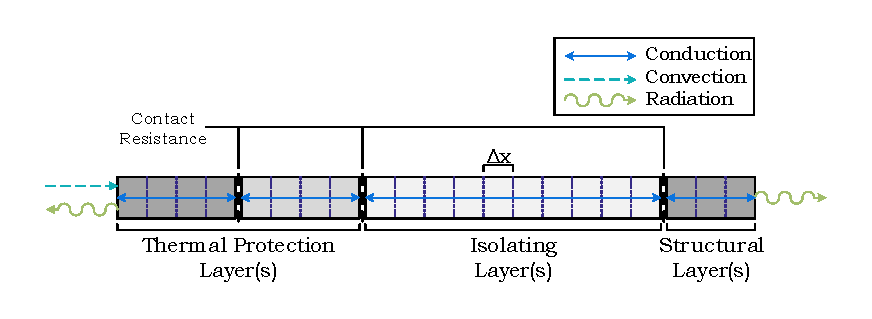
\includegraphics{./Figure/Thermal/1dmodelthermal.pdf}
	\caption{1D thermal model}
	\label{fig:1dmodelthermal}
\end{figure}

Since a 1D thermal model is used to analyse the problem Equation \ref{eq:thermheat}, also known as the 1D heat equation, can be used to relate temperature, space and time using the thermal diffusivity ($\gls{sym:alphat}$). The thermal diffusivity is a function of the thermal conductivity ($\gls{sym:k}$), density ($\gls{sym:rho}$) and specific heat capacity ($\gls{sym:cp}$) as shown in Equation \ref{eq:thermdif} \cite{Holman2002}. A Crank-Nicolson scheme is used to implement the heat equation. This will model the heat conduction within each layer. The convective heating is obtained from the aerodynamic analysis and the radiation is calculated using Equation \ref{eq:thermrad} \cite{Holman2002}. It is assumed that the temperature ($\gls{sym:T}_\infty$) of the gas into which the heat shield radiation is directed, is equal to the atmospheric temperature of Mars.

\vspace{-12px}
\begin{tabular}{lll}
	\begin{minipage}{0.24\linewidth}
	\begin{equation}
	\frac{\partial \gls{sym:T}}{\partial \gls{sym:t}} = \gls{sym:alphat}\frac{\partial^2\gls{sym:T}}{\partial \gls{sym:x}^2}
	\label{eq:thermheat}
	\end{equation}
	\end{minipage}
	&
	\begin{minipage}{0.26\linewidth}
	\vspace{16.5px}
	\begin{equation}
	\gls{sym:alphat} = \frac{\gls{sym:k}}{\gls{sym:rho}\gls{sym:cp}}
	\label{eq:thermdif}
	\end{equation}
	\end{minipage}
	&
	\begin{minipage}{0.4\linewidth}
	\vspace{12px}
	\begin{equation}
	\gls{sym:qdot}_r = \gls{sym:eps}\gls{con:stefanboltzmann}\left(\gls{sym:T}_w^4-\gls{sym:T}_\infty^4\right)
	\label{eq:thermrad}
	\end{equation}
	\end{minipage}
\end{tabular}

\paragraph{Limitations}
Simplifying the problem introduces some limitations to the design tool. One of the drawbacks of a 1D analysis is that the complete \gls{tps} is sized according to the conditions at the stagnation point. Furthermore it does not account for cross-planar heat flow. These drawbacks will decrease the estimated heat through the lay-up and therefore the current analysis method provides a conservative estimate for the \gls{tps}. 

The influence of the assumption that material properties do not vary with temperature on the required thicknesses of different lay-ups is small. Note that this will not lead to a more conservative design as the thermal resistance decreases as temperature increases. 

The paper by Del Corso et al. states that it is difficult to analytically determine the contact resistance \cite{Corso2009}. Del Corso et al. used their own data for this, though arbitrary multiplication factors had to be applied to match their model with the validation data. Also analytically calculating the contact resistance introduces more unknowns that have to be determined. Therefore varying conductivities have been empirically assigned to the thin layers of air between the layers. A disadvantage is that multiple layers had to be tested to find correct conductivities such that the developed tool matches experimental data. The experimental data found in the papers by Del Corso et al. is used for the validation of the thermal model \cite{Corso2009,Corso2011}. The thermal model was successfully verified and validated as shown extensively in Appendix \ref{sec:VandVthermo}.